This chapter aims to present the results of the experiments conducted across Rahguzar’s clustering, scheduling, and routing phases to evaluate their impact on route optimization, workload balancing, and service coverage. Each algorithm was tested individually and as part of the integrated pipeline. Additionally, Rahguzar’s performance was benchmarked against Salesflo using real distributor datasets, comparing outcomes in terms of total travel distance, execution time, and overall planning efficiency.

\section{Algorithmic Phases and Experiment Results}

This section presents the methodology and results from a series of experiments conducted to determine the optimal combinations of algorithms for different phases of the optimization process.




\subsection{Phase 1: Hybrid Clustering Approach}
% Phase 1 content to be added later.
The first aim of the algorithm is to divide the list of stores to be serviced into a number of clusters which is determined by the number of orderbookers.
The objective is to group close stores in the same cluster, so that the orderbookers can service them as the scheduler will decide.
To achieve this, clustering algorithms were tested on their own adn in a hybrid approach.

\subsubsection{Clustering Algorithms Tested}

The following clustering algorithms were evaluated for grouping stores among orderbookers based on geographical proximity and workload balancing:

\begin{itemize}
    \item \textbf{KMeans Clustering}  
    
    Groups stores based on latitude and longitude using the KMeans algorithm. It minimizes the sum of squared distances to cluster centroids. After initial clustering, stores are reallocated from overloaded to underloaded clusters to ensure balanced workload distribution.

    \item \textbf{Hierarchical Clustering}  
    
    This method uses Ward’s linkage to merge clusters based on minimum variance increase. Clusters are formed by cutting the dendrogram at the level corresponding to the number of orderbookers, resulting in compact and cohesive geographic groupings.

    \item \textbf{Gaussian Mixture Models}  
    
    Clusters are modeled as Gaussian distributions with flexible shapes and orientations. Stores are assigned to clusters based on their probability of belonging to a particular Gaussian component. The model uses “full” covariance to allow for non-spherical clusters.

    \item \textbf{Hybrid Approach 1 (Graph-Based Clustering + KMeans)}  
    
    This approach begins by forming clusters based on graph connectivity within a specific distance threshold. These clusters are then refined using KMeans to match the desired number of clusters, ensuring both geographic cohesion and count alignment.

    \item \textbf{Hybrid Approach 2 (Graph-Based Clustering + KMeans + Geographical Constraints)}  
    
    This builds on Hybrid 1 by identifying and reassigning outlier stores. Outliers are detected based on their distance from the cluster centroid exceeding a defined threshold. These stores are then reassigned to the nearest appropriate cluster to enhance geographic cohesion and workload balance.
\end{itemize}


Moreover, to ensure that optimal clusters were being made, cluster balancing was employed to redistribute 
stores between clusters to ensure workloads—based on service effort and travel time—are roughly equal.
 Overloaded clusters transfer nearby stores to underloaded ones, and this process repeats until workloads fall within a set tolerance or a maximum number of iterations is reached, promoting fair and efficient distribution.

\subsection{Phase 1: Experiments Results}
The silhouette score measures how well points are grouped in a clustering task. It checks if points are close to others in their own cluster, indicating a good score, or if they are far from points in other clusters (also good score). The score ranges from -1 to 1, where 1 means perfect clusters, 0 means overlap, and negative scores indicate that points might be in the wrong cluster.

\begin{table}[H]
    \centering
    \resizebox{\textwidth}{!}{%
    \begin{tabular}{|c|c|c|c|c|c|}
    \hline
    \textbf{Distributor ID} & \textbf{KMeans} & \textbf{Gaussian Mixture Models} & \textbf{Hierarchical} & \textbf{Hybrid Approach-1} & \textbf{Hybrid Approach-2} \\
    \hline
    1 & 0.3537 & 0.2835 & 0.3537 & 0.5044 & 0.5044 \\
    6 & 0.1839 & 0.2130 & 0.1839 & 0.1839 & 0.1684 \\
    7 & 0.2737 & 0.3376 & 0.3892 & 0.3980 & 0.4437 \\
    \hline
    \end{tabular}%
    }
    \caption{Silhouette Score Comparison for Different Clustering Algorithms}
    \label{tab:silhouette_scores}
    \end{table}

    \begin{figure}[ht]
        \centering
        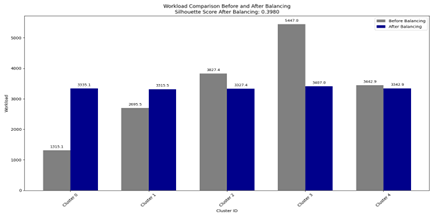
\includegraphics[width=0.75\textwidth]{images/7.1.2 hybrid 1 workload.png}
        \caption{Hybrid Approach-1: Workload Distribution across Clusters}
        \label{fig:hybrid1_workload}
    \end{figure}
    
    \begin{figure}[ht]
        \centering
        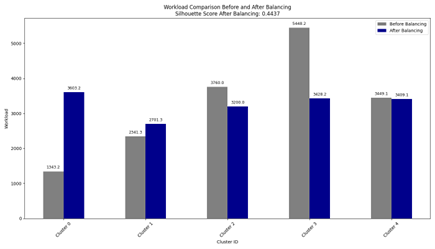
\includegraphics[width=0.75\textwidth]{images/7.1.2 hybrid 2 workload.png}
        \caption{Hybrid Approach-2: Workload Distribution across Clusters}
        \label{fig:hybrid2_workload}
    \end{figure}

% From the results in Table~\ref{tab:silhouette_scores}, it can be observed that the Hybrid Approach-2 outperformed all other clustering algorithms, achieving the highest silhouette score of 0.5044 for Distributor 1 and 0.4437 for Distributor 7. This indicates that the clusters formed using this approach were more cohesive and well-separated compared to those formed by the other algorithms.
% Moreover, it finds a good balance between workload distribution and geographic proximity. For example, for distributor ID 7, there's a little variance in the clusters being formed however, it has the highest silhouette score as geographical proximity has been set as the priority.
From the results in Table~\ref{tab:silhouette_scores}, it can be observed that the Hybrid Approach-2 outperformed all other clustering algorithms, achieving the highest silhouette score of 0.5044 for Distributor 1 and 0.4437 for Distributor 7. This indicates that the clusters formed using this approach were more cohesive and well-separated compared to those formed by the other algorithms.

Figures~\ref{fig:hybrid1_workload} and~\ref{fig:hybrid2_workload} present a visual comparison of workload distribution across clusters for the two hybrid approaches. While Hybrid Approach-1 shows a slightly more uniform distribution of workload, we ultimately prefer Hybrid Approach-2. The reason is that, despite the marginally greater variance in workload, it achieves significantly better geographical compactness—an important factor reflected in the higher silhouette scores. Prioritizing geographic proximity helps ensure route optimization and operational feasibility, which outweighs the minor imbalance in workload.

\subsection{Phase 2: Scheduling with Evolutionary Algorithm (EA)} %
Once clusters have been formed in Phase 1, the next critical step is to generate a feasible schedule that defines which shops should be visited on each day of the planning period (either a single day or a custom range, as selected by the user). The primary objective during scheduling is to balance the workload across both the available days and all assigned orderbookers. This ensures that no orderbooker is disproportionately burdened and that their daily tasks are distributed as evenly as possible.

To identify the most effective scheduling strategy, a series of experiments were conducted using various algorithms. Each algorithm was evaluated based on its ability to generate balanced, constraint-compliant schedules. At the core of this evaluation process is the fitness function.

The fitness function plays a vital role in determining how practical and efficient a schedule is. It computes a cost value for each candidate schedule—lower values indicate better solutions. Hard constraints are applied first: for example, if the total route time on any day exceeds a predefined daily limit (e.g., 480 minutes), a substantial penalty is applied to immediately discourage infeasible schedules. It also checks for visit mismatches—stores not visited the required number of times—penalizing any deviations.

Additionally, soft constraints are incorporated to further refine the schedule. These include a day-balancing penalty when daily route times fall outside the ideal range (e.g., 360–420 minutes), and a geographical penalty when neighboring stores requiring only one visit are assigned to different days. These constraints collectively guide the algorithm toward generating schedules that are not only valid but also optimized for balance, practicality, and real-world efficiency. The following scheduling algorithms were used:

\begin{itemize}
    \item Simulated Annealing
    \item Ant Colony Optimization (ACO)
    \item Mixed Integer Linear Programming (MILP)
    \item Evolutionary Algorithm (EA)
\end{itemize}

Through a series of experiments, the best combination for the scheduling phase was determined, which was Evolutionary Algorithm (EA) for scheduling.
Algorithms like ACO showed that the in serach for the optimal schedule, it can often get trapped in a local optima. For MILP and simulated annealing, 
generating a schedule can be computationally expensive and time consuming. On the other hand, EA showed optmial results with genetic diversity maintained that
avoids premature convergence, hence EA is the best choice for scheduling.

\subsection{Phase 3: Route Optimization}
After a schedule has been created, the next step is to optimize the routes for each orderbooker. This involves determining the most efficient path for each orderbooker to follow, ensuring that they can visit all assigned stores in the shortest possible time while adhering to any constraints (e.g., time windows, vehicle capacity). The goal is to minimize travel distance and time while maximizing efficiency. This phase is crucial for ensuring that the orderbookers can complete their routes within the allocated time and resources, ultimately leading to improved service levels and reduced operational costs.

Moreover, it helps determine the order of visiting the stores and the best route to take, considering factors such as road networks and other logistical constraints. For route optimization, several algorithms were tested to identify the most effective one. The route optimization algorithms evaluated were:

\begin{itemize}
    \item Particle Swarm Optimization (PSO)
    \item Ant Colony Optimization (ACO)
    \item Google Optimization Tools (OR-Tools)
    \item Evolutionary Algorithm (EA)
    \item Dynamic Programming
\end{itemize}

Among the tested route optimization algorithms, Google OR-Tools showed the most consistent and optimal performance in minimizing total travel distance and time. While ACO and PSO showed promise in smaller test cases, they frequently got trapped in local optima or exhibited longer computation times in large-scale datasets. OR-Tools, by contrast, delivered high-quality solutions across varying distributor profiles and constraints, making it the most robust choice for route optimization within Rahguzar's pipeline.




\subsection{Phase 2 and 3: Experiments Overview}
A series of experiments were conducted across different distributors with varying numbers of stores and orderbookers. The following distributors were involved in the experiments:
\begin{table}[h!]
\centering
\begin{tabular}{|c|c|c|}
\hline
\textbf{Distributor ID} & \textbf{Number of Stores} & \textbf{Number of Orderbookers} \\
\hline
1 & 395 & 2 \\
6 & 426 & 4 \\
7 & 580 & 5 \\
131 & 42 & 1 \\
\hline
\end{tabular}
\caption{Distributors and their Assigned Stores and Orderbookers}
\end{table}

The purpose of the experiments was to determine the best combinations of scheduling and route optimization algorithms for each distributor. The experiments were designed to evaluate the performance of different algorithmic combinations in terms of distance and travel time minimization.
This was done by analyzing the total distance and the total traveltime minimized across all orderbookers (results show average of all distributors), and the stores serviced distribution per orderbooker for each day.

\begin{figure}[H]
    \centering
    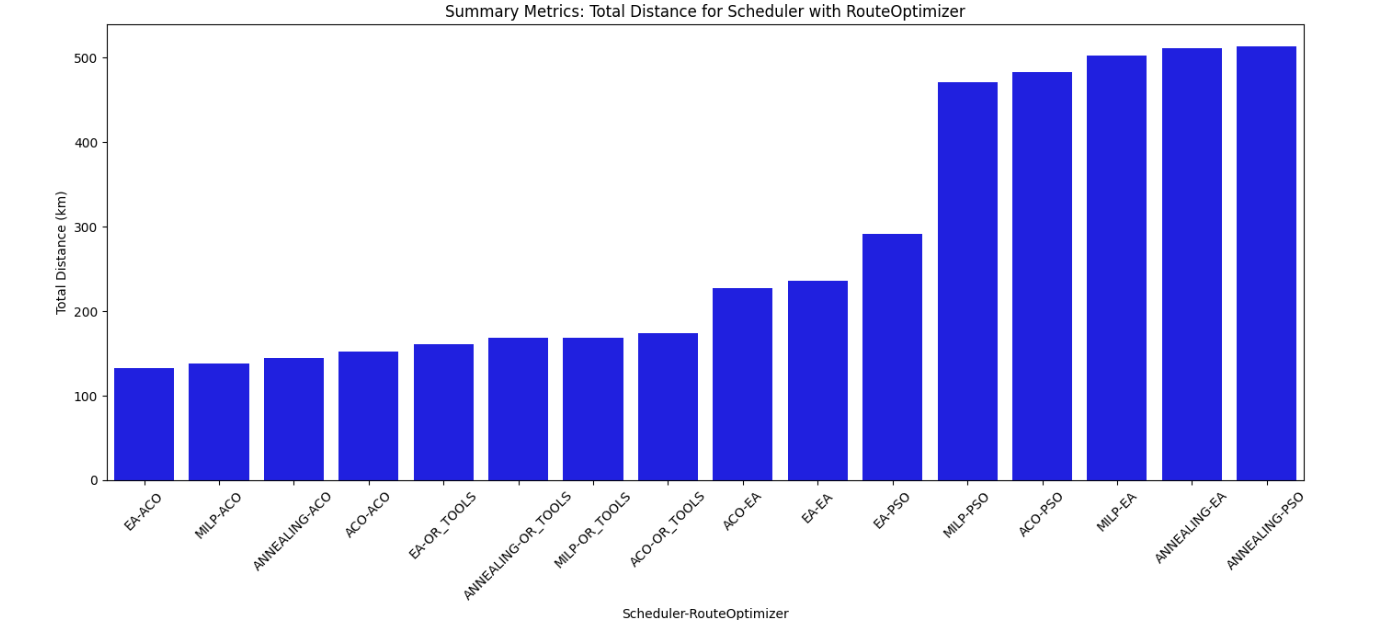
\includegraphics[width=0.95\textwidth]{images/results_distance_all_dis}
    \caption{Total distance for all distributors compared over different combinations.}
    \label{fig:results_distance_all_dis}
\end{figure}

\begin{figure}[H]
    \centering
    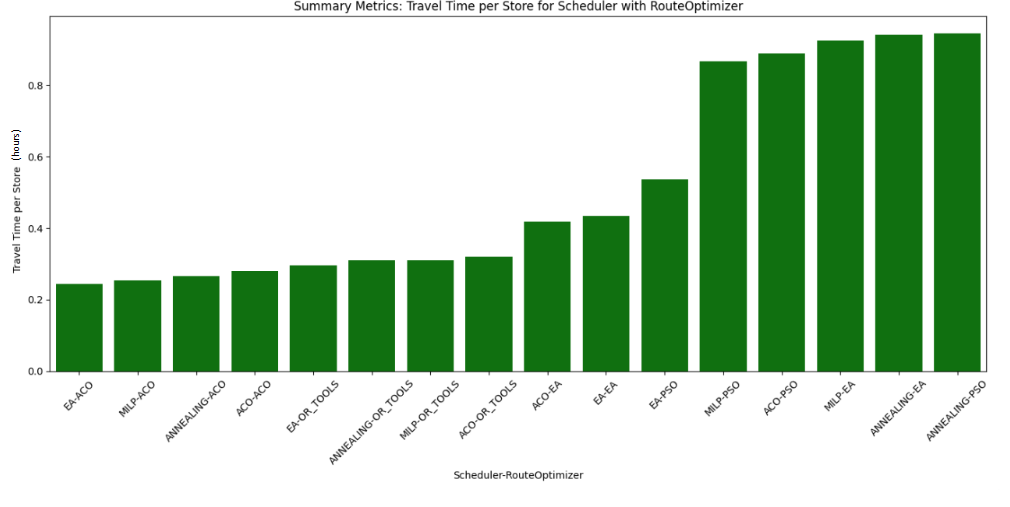
\includegraphics[width=0.95\textwidth]{images/results_time_all_dis}
    \caption{Total time for all distributors compared over different combinations.}
    \label{fig:results_time_all_dis}
\end{figure}

The results in Figure~\ref{fig:results_distance_all_dis} and Figure~\ref{fig:results_time_all_dis} show that one of the top-performing scheduler-route optimizer combinations was EA-OR Tools, which demonstrated strong results in minimizing both travel distance and time, by traveling 
to as less as 150 km in 0.2 hours, as compared to almost 500 kms and 1 hour for the worst combination. OR Tools consistently ranked among the top-performing route optimizers across multiple test cases, whereas the least optimal performance was showed EA nad PSO route optimizers, 
and MILP and simulated annealing schedulers.


\subsection{Phase 2 and 3: Experiment Results}
The experiments were conducted by combining different scheduling algorithms with different route optimization algorithms. The findings of each graph is summarized below.



The best performing scheduler-route optimizer combinations for each distributor are as follows:

\begin{table}[H]
    \centering
    \renewcommand{\arraystretch}{1.3}
    \caption{Best Performing Scheduler-Route Optimizer Combinations by Distributor}
    \begin{tabular}{|>{\centering\arraybackslash}p{4cm}@{\hskip 0.5cm}|>{\centering\arraybackslash}p{5cm}@{\hskip 0.5cm}|>{\centering\arraybackslash}p{5cm}|}
    \hline
    \textbf{Distributor} & \textbf{Best Distance Minimized Scheduler-Route Optimizer} & \textbf{Best Travel Time Minimized Scheduler-Route Optimizer} \\
    \hline
    Distributor 7 & EA-OR-Tools & EA-OR-Tools \\
    Distributor 6 & EA-OR-Tools & EA-OR-Tools \\
    Distributor 1 & EA-OR-Tools & EA-OR-Tools \\
    Distributor 131 & EA-ACO & EA-ACO \\
    \hline
    \end{tabular}
    \label{tab:best_schedulers}
\end{table}


    
\section{Results Comparison: Salesflo PJP vs Rahguzar PJP}

This section presents a comparative analysis of Rahguzar's performance against Salesflo's pre-existing PJP plans across three real-world test distributors. Each distributor varied in terms of store count, OB allocation, and planning duration, allowing for a diverse evaluation of route efficiency, time optimization, and system scalability. Metrics analyzed include total distance traveled and total route time under the same operational constraints for both systems.

\subsection{Test Distributor 1 – Results Comparison}

To evaluate Rahguzar’s performance, the first distributor involved 365 stores serviced by 2 Order Bookers (OBs) over a 3-day plan. The results are summarized below:

\begin{table}[H]
\centering
\caption{Performance Comparison – Test Distributor 1}
\renewcommand{\arraystretch}{1.3}
\begin{tabular}{|>{\centering\arraybackslash}p{4cm}@{\hskip 0.5cm}|>{\centering\arraybackslash}p{3.2cm}@{\hskip 0.5cm}|>{\centering\arraybackslash}p{3.2cm}|}
\hline
\textbf{Metric} & \textbf{Salesflo} & \textbf{Rahguzar} \\
\hline
Total Shops & 365 & 365 \\
Order Bookers & 2 & 2 \\
Plan Duration (days) & 3 & 3 \\
Total Distance (km) & 227.87 & 218.77 \\
Total Time (hrs) & 35.53 & 35.39 \\
\hline
\end{tabular}
\label{tab:dist1_comparison}
\end{table}

Rahguzar reduced the total travel distance by \textbf{9.1 km} and total time by \textbf{0.14 hours}, reflecting modest spatial and temporal efficiency.

\subsection{Test Distributor 2 – Results Comparison}

The second distributor included 1153 stores and 3 OBs over a 6-day schedule:

\begin{table}[H]
\centering
\caption{Performance Comparison – Test Distributor 2}
\renewcommand{\arraystretch}{1.3}
\begin{tabular}{|>{\centering\arraybackslash}p{4cm}@{\hskip 0.5cm}|>{\centering\arraybackslash}p{3.2cm}@{\hskip 0.5cm}|>{\centering\arraybackslash}p{3.2cm}|}
\hline
\textbf{Metric} & \textbf{Salesflo} & \textbf{Rahguzar} \\
\hline
Total Shops & 1153 & 1153 \\
Order Bookers & 3 & 3 \\
Plan Duration (days) & 6 & 6 \\
Total Distance (km) & 929.25 & 545.01 \\
Total Time (hrs) & 113.77 & 108.54 \\
\hline
\end{tabular}
\label{tab:dist2_comparison}
\end{table}

Rahguzar achieved a reduction of \textbf{384.24 km} in distance and \textbf{5.23 hours} in time, demonstrating high scalability and optimization capability.

\subsection{Test Distributor 3 – Results Comparison}

This case involved 659 stores and 2 OBs, also over a 6-day cycle:

\begin{table}[H]
\centering
\caption{Performance Comparison – Test Distributor 3}
\renewcommand{\arraystretch}{1.3}
\begin{tabular}{|>{\centering\arraybackslash}p{4cm}@{\hskip 0.5cm}|>{\centering\arraybackslash}p{3.2cm}@{\hskip 0.5cm}|>{\centering\arraybackslash}p{3.2cm}|}
\hline
\textbf{Metric} & \textbf{Salesflo} & \textbf{Rahguzar} \\
\hline
Total Shops & 659 & 659 \\
Order Bookers & 2 & 2 \\
Plan Duration (days) & 6 & 6 \\
Total Distance (km) & 143.66 & 142.46 \\
Total Time (hrs) & 58.95 & 58.99 \\
\hline
\end{tabular}
\label{tab:dist3_comparison}
\end{table}

Rahguzar reduced the distance by \textbf{1.2 km}, with a slight increase in time of \textbf{0.04 hours}, indicating comparable efficiency.

\subsection{Summary Across All Distributors}

To illustrate overall performance across all scenarios:

\begin{table}[H]
\centering
\caption{Combined Performance Summary}
\renewcommand{\arraystretch}{1.3}
\begin{tabular}{|>{\centering\arraybackslash}p{2cm}@{\hskip 0.4cm}|>{\centering\arraybackslash}p{3.4cm}@{\hskip 0.4cm}|>{\centering\arraybackslash}p{4cm}@{\hskip 0.4cm}|>{\centering\arraybackslash}p{3.2cm}|}
\hline
\textbf{Distributor} & \textbf{Platform} & \textbf{Total Distance (km)} & \textbf{Total Time (hrs)} \\
\hline
1 & Salesflo & 227.87 & 35.53 \\
  & Rahguzar & 218.77 & 35.39 \\
\hline
2 & Salesflo & 929.25 & 113.77 \\
  & Rahguzar & 545.01 & 108.54 \\
\hline
3 & Salesflo & 143.66 & 58.95 \\
  & Rahguzar & 142.46 & 58.99 \\
\hline
\end{tabular}
\label{tab:combined_summary}
\end{table}

Across all test cases, Rahguzar reduced the cumulative travel distance by \textbf{540.79 km} and time by \textbf{5.41 hours}, validating its effectiveness in optimizing field operations.

\begin{figure}[H]
    \centering
    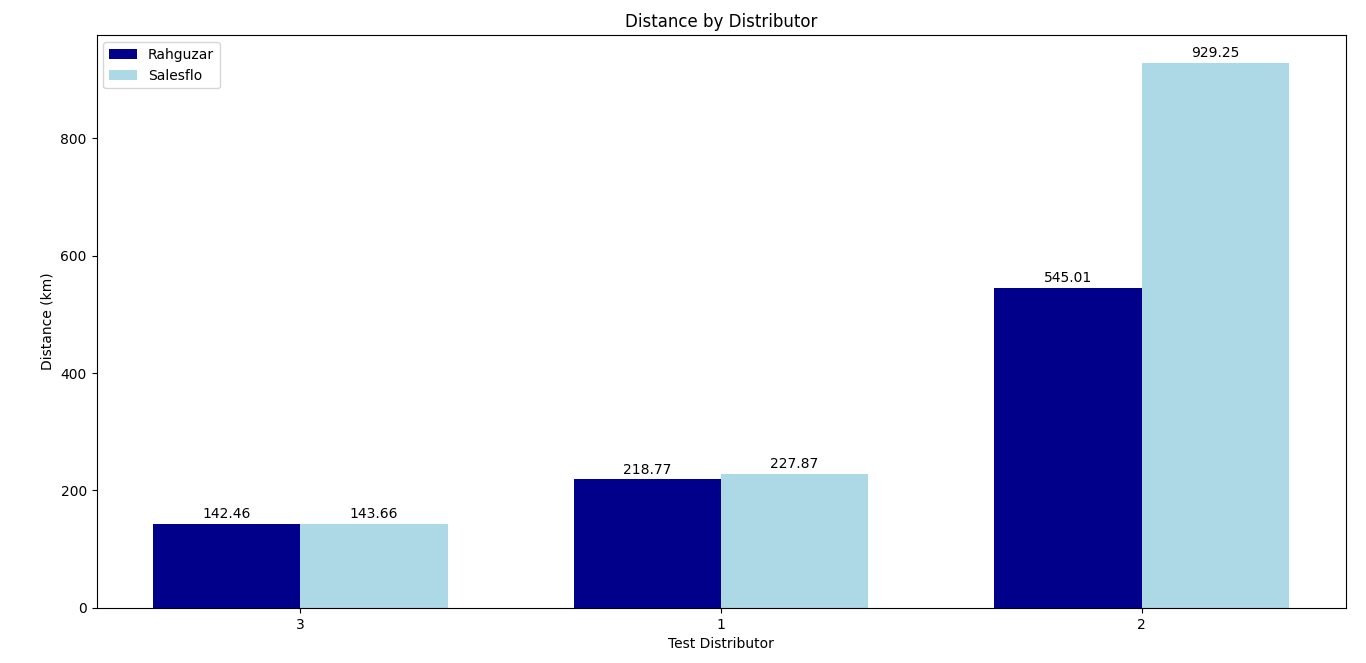
\includegraphics[width=0.95\textwidth]{images/distance_rahgyzar_salesflo_comp}
    \caption{Total distance comparision for the test distributors.}
    \label{fig:results_distance_comparision}
\end{figure}


\begin{figure}[H]
    \centering
    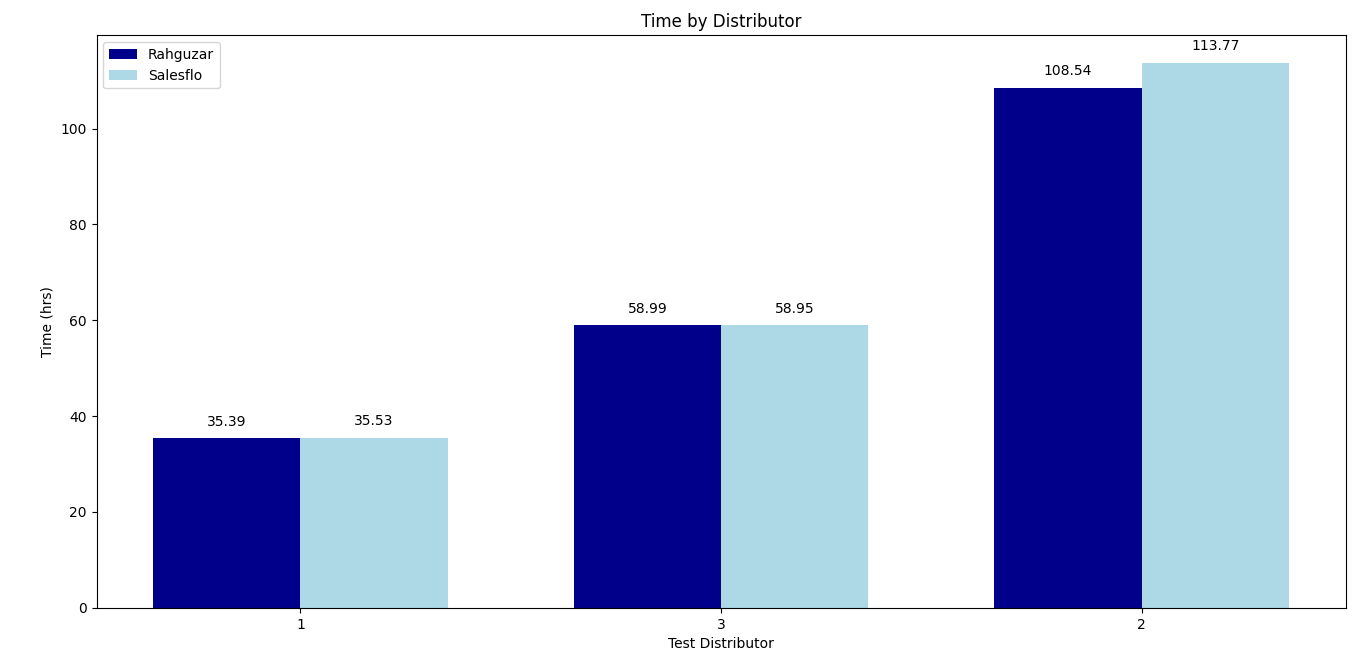
\includegraphics[width=0.95\textwidth]{images/time_rahgyzar_salesflo_comp}
    \caption{Total time comparision for the test distributors}
    \label{fig:results_time_comparision}
\end{figure}


Based on the results of the experiments, the Evolutionary Algorithm (EA) consistently demonstrated strong performance in the scheduling phase, effectively balancing workloads and meeting visit constraints across varying distributor profiles. For route optimization, Google OR-Tools emerged as the most robust and scalable solution, outperforming other algorithms—including ACO and PSO—particularly in large-scale and constraint-heavy scenarios.

The combination of EA for scheduling and OR-Tools for routing provided the most efficient and adaptable pipeline, delivering optimal results in both distance and time minimization. This pairing proved especially effective in consistently handling real-world distributor datasets.

Furthermore, when benchmarked against Salesflo, Rahguzar showed clear improvements in planning efficiency, with notable reductions in total distance traveled and route time. These findings highlight Rahguzar’s potential as a scalable and intelligent planning system that can adapt to operational complexity while delivering measurable gains in field performance.